\begin{figure}[b]
\centering
  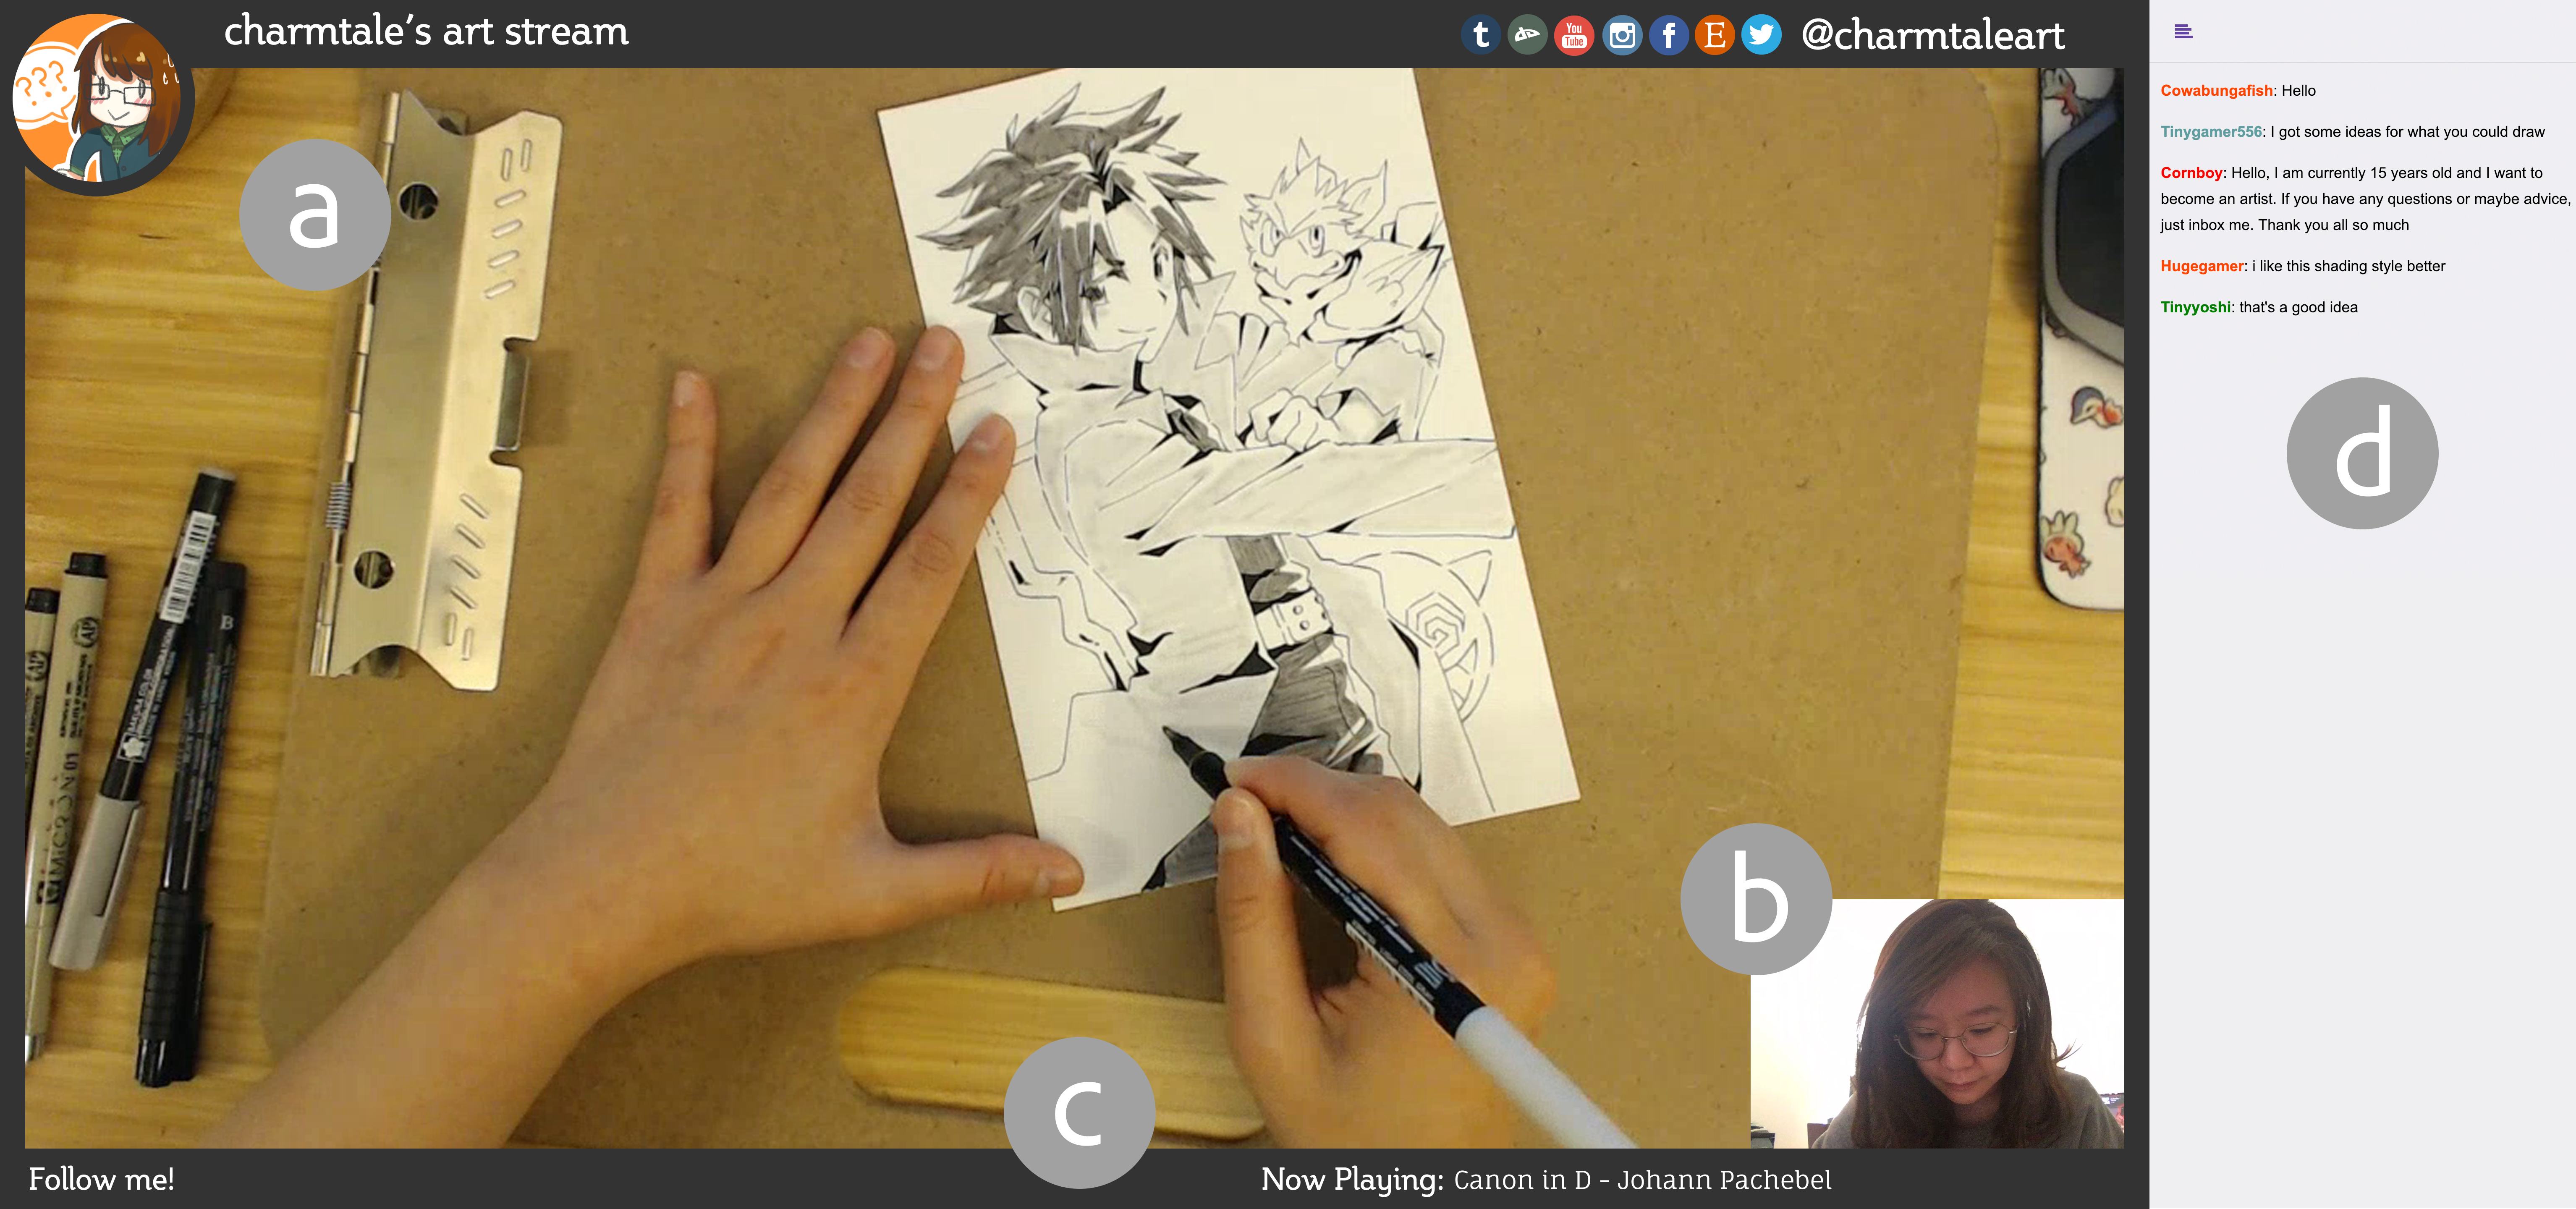
\includegraphics[width=1\columnwidth]{livestreams/figures/livestreaming_paper_figure_anonymized.jpg}
  \caption{A typical creative livestream setup. (a) A camera or screencast displays the artist's workspace. (b) A second camera shows the artist's face. (c) Graphical overlays provide ambient information about the artist (\textit{e.g.,} social media pages) and display interactions with the audience (\textit{e.g.,} pop-ups that appear when viewers subscribe or donate to the stream). (d) Live chat allows viewers to communicate with the streamer. }~\label{fig:livestreaming_view}
  \vspace{-0.15in}
\end{figure}

\section{What are creative livestreams?}
Popular livestreaming platforms include Twitch, YouTube, Facebook, Instagram, and Periscope. Picarto, a livestreaming platform dedicated to creative work, launched in 2013. Twitch launched its \textit{Creative} category in 2015 \cite{Moorier2015}. To deal with its explosion in popularity, Twitch replaced the \textit{Creative} category with six more-specific categories in September 2018: \textit{Art}, \textit{Music \& Performing Arts}, \textit{Science \& Technology}, \textit{Beauty \& Body Art}, \textit{Food \& Drink}, and \textit{Makers \& Crafting} \cite{Robertson2018}. 
%\xxx{Also, would it be interesting to note the \# of streamers or avg \# of streams in that category?}\xxx{can't get those numbers via the twitch api. figure 2 is the best i could do} 
%\xxx{I agree with xxx. Why is Twitch the one platform you call out here?} \xxx{i mention youtube and picarto below (moved picarto up sooner), is there something more i should say? can't isolate creative streams with certainty on youtube. can't find a usable \textsc{api} for periscope. } 
Creative livestreams also appear on many other platforms, but often without a distinct category. For example, many creative streams on YouTube are categorized as \textit{Education}, \textit{How-to \& Style}, or even \textit{Gaming}.

Livestream videos (\autoref{fig:livestreaming_view}) typically show the artist's full screen (when working on a computer) or workspace (for physical work) and a camera view of their face. Livestreams usually also feature a live chat, allowing viewers to communicate with each other and the artist. 

To learn more about creative livestreams, we studied two popular platforms: Twitch and YouTube. As these large platforms cover many types of content, we narrowed our investigation to the \textit{Creative} category on Twitch and the \textit{Adobe Live} video series on YouTube. Through this, we see how streams and communities differ across platforms.  
%For example, on Twitch anyone is welcome to stream, while Adobe invites special guest artists to their studio. On Twitch its up to each artist to make their stream engaging, while Adobe invites hosts to help engage with the audience. 
%This section provides an overview of two popular creative livestreaming communities: the Creative category on Twitch, and livestreams hosted by Adobe. We focus on these communities as they are hosted through popular platforms (Twitch and YouTube), which are the two most frequently-mentioned platforms by survey respondents who watch creative livestreams.

\subsection{Creative livestreams on Twitch: Content analysis}
To better understand the format and content of creative live\-streams, we analyzed a sample of videos on Twitch, one of the most popular platforms for livestreaming. For each creative category, we gathered aggregate metrics about streamers and viewers. We watched and took notes on a sample of 29 videos. We identified four common types of creative livestreams that will appear throughout the paper: \textit{Teaching}, \textit{Making}, \textit{Socializing}, and \textit{Performing}.

\subsubsection{Methodology}
To measure the popularity and activity in each of the six creative categories, we queried the Twitch \textsc{api} 4 times a day for 7 days to obtain the number of currently-live streams and number of currently-watching viewers in each category.

We also used the Twitch \textsc{api} to download metadata about the videos in each category (limited to top 600)
%Because this \textsc{api} halts video requests after 600 videos, so our script downloaded metadata for the 600 most-viewed videos in each category. The script 
and randomly selected 50 archived English livestream videos. Four annotators (including the first author) watched each of these videos. Ten videos were not available for viewing and thus excluded (either because their archive expired between being downloaded and being annotated, or because they were only available to subscribers of a channel). Another 11 videos were excluded as they showed video games, TV show reruns, or live event coverage. While these videos were categorized as creative on Twitch, they did not reflect our definition of creative work, namely the creation of a novel artifact. This yielded 29 videos. For each, annotators took notes in a structured spreadsheet on the content presented, camera setup, overall structure of the stream, artist's presentation style, and chat activity.

\begin{table}[b]
\centering
\caption{Summary of popularity of Twitch's creative livestream categories. The number of currently-live streams and currently-watching viewers were collected 4 times a day for a week and then averaged.}~\label{table:livestream_summary}
\begin{tabular}{llll}
\textbf{Category}        & \textbf{\begin{tabular}[c]{@{}l@{}}Avg. \#\\ livestreams\end{tabular}} & \textbf{\begin{tabular}[c]{@{}l@{}}Avg. \# live\\ viewers\end{tabular}} & \textbf{\begin{tabular}[c]{@{}l@{}}Avg. \# viewers\\ / stream\end{tabular}} \\
Art                      & 339                                                                    & 6417                                                                    & 21                                                                          \\
Beauty \& Body Art       & 5                                                                      & 177                                                                     & 17                                                                          \\
Food \& Drink            & 19                                                                     & 1088                                                                    & 64                                                                          \\
Makers \& Crafting       & 40                                                                     & 680                                                                     & 16                                                                          \\
Music \& Performing Arts & 286                                                                    & 6881                                                                    & 24                                                                          \\
Science \& Technology    & 91                                                                     & 1155                                                                    & 12                                                                         
\end{tabular}
\end{table}

While this sample does not capture all types of creative activities one might livestream, our hope is that by analyzing a set of canonically creative activities we can shed light on a broader set of activities that might also have a creative component (\textit{e.g., } video games that involve creating artifacts).
%There is overlap among categories on Twitch, even sometimes within a single livestream when an artist switches back and forth between creative work and other activities like gaming. 

\subsubsection{Results: Most streamers focus on work \& engage with viewers}
\autoref{table:livestream_summary} shows overall metrics for the creative categories on Twitch. The most popular categories by far are \textit{Art} and \textit{Music \& Performing Arts}. The category with the most viewers watching per stream is \textit{Food \& Drink}, likely because there are fewer streams to choose from relative to the number of interested viewers. These communities are small relative to the most popular games; for example, the game Fortnite has between 5,000 and 10,000 streams live on Twitch at any given time, with around 100,000 total viewers watching. %\xxx{xxx says move earlier but where?}

\begin{table}[b!]
\centering
\caption{Creative activities shown in a random sample of 29 livestreams from Twitch's creative categories, and the primary type of structure each stream exhibits.}~\label{table:livestream_activities}
\begin{tabular}{lll}
\textbf{Category}        & \textbf{Activity (\# videos if \textgreater 1)} & \textbf{\begin{tabular}[t]{@{}l@{}}Primary type\\ of stream\end{tabular}} \\
Art                      & Multimedia production                           & Making                                                                    \\
                         & Digital drawing (4)                             & Making                                                                    \\
                         & Animation                                       & Teaching                                                                  \\
                         &                                                 &                                                                           \\
Beauty \& Body Art       & Makeup                                          & Socializing                                                               \\
                         & Makeup (3)                                      & Making                                                                    \\
                         &                                                 &                                                                           \\
Food \& Drink            & Cooking                                         & Teaching                                                                  \\
                         &                                                 &                                                                           \\
Makers \& Crafting       & Making foam props                               & Teaching                                                                  \\
                         & Sewing quilts                                   & Socializing                                                               \\
                         & Bead art (2)                                    & Making                                                                    \\
                         & Assembling models                               & Making                                                                    \\
                         & Assembling models                               & Socializing                                                               \\
                         & Woodworking                                     & Making                                                                    \\
                         & Pottery                                         & Making                                                                    \\
                         &                                                 &                                                                           \\
Music \& Performing Arts & Music production                                & Performing                                                                \\
                         & Music production                                & Making                                                                    \\
                         & Acting \& improv games                          & Performing                                                                \\
                         &                                                 &                                                                           \\
Science \& Technology    & Building a computer                             & Making                                                                    \\
                         & Programming (3)                                 & Making                                                                    \\
                         & Game development (2)                            & Teaching                                                                  \\
                         & Talking about technology                        & Socializing                                                              
\end{tabular}
\end{table}

The videos span a range of creative activities (\autoref{table:livestream_activities}). The average video length was 3h46m, not including time spent gaming -- a few artists combined both creative work and video gaming into one stream, spending the first part on creative work then switching to gaming when they were finished. The shortest video was 1h3m; the longest was 7h56m. These videos are notably longer than most non-livestream videos.

Almost all videos contained either a screencast view for work being done on a computer (13/29) or a camera view for physical work (15/29). One showed a distant camera view of the artist producing music in a studio. Most (26/29) showed the artist's face: in 10 as part of the main camera feed, and 16 as a separate feed overlaid in a corner (as in \autoref{fig:livestreaming_view}). Almost all artists (27/29) talked out loud while streaming; of the two silent streamers, one occasionally posted in the chat. Most artists talked about a mix of their work and other topics (18/29). Some talked only about their work (9), or only about other topics (1). One was a variety show, so the talking \textit{was} the work. Many videos (19/29) included background music. 

Most artists engaged with the chat at least sometimes (24/29). 18 artists engaged frequently with the chat, and 6 occasionally. Three videos did not show a chat replay despite the artist referring to the chat; we assume it was not saved or had been hidden. In all 26 remaining videos, viewers asked questions at least occasionally, or in some videos (9/26) frequently. In half of these videos, all chat questions appeared to get answered; in the rest, some (7/13) or many (4/13) questions went unanswered. In 2 videos, most chat questions were answered by other viewers or moderators in the chat.

\subsubsection{Four common types of creative livestreams}
We identified four common types of creative livestreams. We also observed these in interviews with streamers in the next section. Sj{\"{o}}blom \textit{et al.} \cite{Sjoblom2017a} offer a similar characterization of video game livestreams; we found some key differences and fewer overall types of structures. \autoref{table:livestream_activities} shows the primary type of each stream in our sample set. These are general high-level trends; some streams bridge multiple types.

\textbf{Teaching} streams have an instructional focus, where the stream\-er is educating the viewers. These include step-by-step how-to demonstrations of tasks such as cooking a recipe, producing a photo-editing effect, or creating DIY costumes. Other examples include critiquing others' work, answering viewers' questions, or explaining a topic.

\textbf{Making} streams focus primarily on creative work and process, but not explicit teaching. These include an artist silently drawing, a streamer attempting a new task they have not tried before and talking their way through it, and an artist making pottery and describing \textit{what} they are doing but not \textit{how}. 

\textbf{Socializing} streams feature the streamer chatting casually with viewers, often while working on a project, such as makeup or sewing (but the project is not the main focus). These are often described as ``chill'' streams. Socializing streams often have tight-knit communities; the streamer will recognize the names of viewers in the chat and ask them how they are doing.

\textbf{Performing} streams feature the artist performing their work. Naturally, these mostly include performative arts like music and acting (\textit{e.g.,} as opposed to drawing). Like with Making, the focus is on the artist's work; in this case the artist does not talk about what they are doing, they just do it. Performing streams differ from non-live recordings in that they often take a more casual improvisational form, rather than scripted performance (\textit{e.g.,} musical ``jam sessions'' or improv acting).

Within each type, the amount of interaction between the stream\-er and the audience varies. Some streamers hold ``request streams'' or ``Q\&A streams'', where the content and flow are determined by audience requests or questions, respectively. Some hold contests or games. A request stream could have audience members requesting songs for a Performing stream, a topic for a Teaching stream, or a particular artifact for the artist to make in a Making or Socializing stream. 

\subsection{Creative livestreams go professional}
While many livestreams are run by individuals, professionally-run livestreams are also growing in popularity. Adobe, a company that produces creative software, hosts livestreams on a regular schedule multiple times a week\footnote{\href{https://behance.net/live}{\nolinkurl{behance.net/live}}}. These can be viewed on Behance or on Adobe's Creative Cloud YouTube channel. They host two livestream series: \textit{Adobe Live} is a Making stream that happens for 6 hours (three 2-hour sessions) three days a week, and it features guest artists usually hosted by someone who works at Adobe. \textit{Daily Creative Challenges} is a Teaching stream that happens for 30 minutes five days a week. It complements contests organized by Adobe to teach new skills. YouTube reports these streams having between 2,000 and 8,000 views each; it does not distinguish between live and replayed views.

\stepcounter{footnote}
\begin{figure}[b]
\vspace{-0.1in}
\centering
  \includegraphics[width=1\columnwidth]{livestreams/figures/adobelive.png}
  \caption{The \textit{Adobe Live} series features a guest artist (bottom left) and a host (bottom right). The artist is working on a digital drawing, and the host is looking up at the live chat feed, engaging with the audience (\href{https://youtu.be/yYDmQhg_1uE}{\nolinkurl{youtu.be/yYDmQhg_1uE}}). }~\label{fig:livestream_adobelive}
  \vspace{-0.2in}
\end{figure}

\textit{Adobe Live} differs from most streams by featuring two people. Typically there is a host and an guest artist (\autoref{fig:livestream_adobelive}), but sometimes two artists work together. Adobe hosts different artists every week across a range of creative disciplines (\textit{e.g.,} graphic design, UX design, photography, video editing). Typically, the host moderates the stream, responding to chat messages and passing on questions from viewers to the artist so that the artist can focus on their work. When the stream includes two artists, they trade off hosting.
%xxx: removing for now because we haven't talked about challenges for streamers yet
%These livestreams address some of the challenges self-streamers often face, such as facilitating the chat while working and dealing with technical setup, by having separate people take on those tasks. 
The featured artists are usually practitioners, not teachers; their work mainly serves as inspirational demonstrations, while also giving the the community a chance to engage with questions and comments. 

The \textit{Daily Creative Challenges} series features one person who both reads chat messages and provides a short tutorial on a software technique. These livestreams are part of Adobe's Creative Challenges, which are contests that encourage people to use Adobe software and submit design work for prizes\footnotemark. These streams are 30 minutes long -- this is short for a livestream -- and focus on instruction: explaining the challenge of the day and teaching viewers the skill of the day. 

\footnotetext{\href{https://www.behance.net/dailycreativechallenge}{\nolinkurl{behance.net/dailycreativechallenge}}}

%The interviews and surveys in this paper are with a mix of people from Adobe's livestreams and from other creative communities, allowing us to gain a broad understanding of the challenges creative streamers face and suggest possible improvements for them.